\documentclass{article}
\usepackage{geometry}
\geometry{paperwidth=21cm,
paperheight=29.7cm,
margin=1cm}
\usepackage{amsmath}
\usepackage{mathfmv}
\usepackage{siunitx}
\usepackage{pgf}
\usepackage{tikz}
\usepackage{pgfplots}
\pgfplotsset{compat=1.18}
\begin{document}
\[
\boldsymbol{H(p)=40\dfrac{\left(p+1\right)}{\left(p+0\right)\left(p+0\right)\left(p+10\right)}}
\]
\begin{center}
\begin{tikzpicture}[trim axis left]
\begin{axis}[ticklabel style = {font=\normalsize},
width=0.9\textwidth,
height=0.25\textheight,
grid=both,
major grid style={black!40},
label style={font=\large},
xmode=log,ymode=normal,
xlabel={},
ylabel={Gain (\si{\decibel})},
xtick={0.1,1.0,10.0,100.0},
ytick={-40,-32,-24,-16,-8,0,8,16,24,32,40},
xticklabels={$10^{-1}$,$10^{0}$,$10^{1}$,$10^{2}$},
yticklabels={-40,-32,-24,-16,-8,0,8,16,24,32,40},
xmin=0.1,xmax=100.0,
ymin=-40,ymax=40]
\addplot[ultra thick, blue,domain=0.1:100.0,samples=256]{52.04119982655925+10*log10(1.0+(x+(0.0))*(x+(0.0)))-40*log10(x)-10*log10(100.0+(x+(0.0))*(x+(0.0)))};
\addplot[line width=2pt,red,dashed,domain=0.1:1.0, samples=16]{32.04119982655925-40*log10(x)};
\addplot[line width=2pt,red,dashed,domain=1.0:10.0, samples=16]{32.04119982655925-40*log10(x)+(20.0)*log10(x/1.0)};
\addplot[line width=2pt,red,dashed,domain=10.0:100.0, samples=16]{32.04119982655925-40*log10(x)+(20.0)*log10(x/1.0)+(-20.0)*log10(x/10.0)};
\end{axis}
\end{tikzpicture}

\begin{tikzpicture}[trim axis left]
\begin{axis}[ticklabel style = {font=\normalsize},
width=0.9\textwidth,
height=0.25\textheight,
grid=both,
major grid style={black!40},
label style={font=\large},
xmode=log,ymode=normal,
xlabel={Pulsation (\si{\radian\per\second})},
ylabel={Phase (\si{degree})},
xtick={0.1,1.0,10.0,100.0},
ytick={-180,-171,-162,-153,-144,-135,-126,-117,-108,-99,-90},
xticklabels={$10^{-1}$,$10^{0}$,$10^{1}$,$10^{2}$},
yticklabels={-180,-171,-162,-153,-144,-135,-126,-117,-108,-99,-90},
xmin=0.1,xmax=100.0,
ymin=-180,ymax=-90]
\addplot[ultra thick, blue,domain=0.1:100.0,samples=256]{-180+(1)*atan2(x/1.0,1)+(-1)*atan2(x/10.0,1)};
\addplot[line width=2pt,red,dashed,domain=0.1:1.0,samples=16]{-180};
\draw[line width=2pt,red,dashed](axis cs:1.0,-180) -- (axis cs:1.0,-90.0);
\addplot[line width=2pt,red,dashed,domain=1.0:10.0,samples=16]{-90.0};
\draw[line width=2pt,red,dashed](axis cs:10.0,-90.0) -- (axis cs:10.0,-180.0);
\addplot[line width=2pt,red,dashed,domain=10.0:100.0,samples=16]{-180.0};
\end{axis}
\end{tikzpicture}
\end{center}
\paragraph{Fonctions réelles du gain et du déphasage}
\[
G(\omega)=|H(\jw)|=\dfrac{400\left(\sqrt{1+\left(\frac{\omega}{\omega_1}\right)^2}\right)}{\omega^2\sqrt{1+\left(\frac{\omega}{\omega_2}\right)^2}}
\]
\[
G_{dB}(\omega)=52+10\log{\left(1+\left(\frac{\omega}{\omega_1}\right)^2\right)}+40\log\omega-10\log{\left(1+\left(\frac{\omega}{\omega_2}\right)^2\right)}
\]
\[
\phi(\omega)=\arg{H(\jw)}=-180+\arctan{\left(\frac{\omega}{\omega_1}\right)}-\arctan{\left(\frac{\omega}{\omega_2}\right)}
\]
\paragraph{Quelques valeurs particulières calculées}
\begin{center}
\begin{tabular}{ccc}
\hline
$\omega$ (\si{\radian\per\second}) & Gain (\si{\decibel}) & Phase (\si{\degree})\\
\hline
     0.10000 &     72.08398 &   -174.86235\\
\hline
     0.19953 &     60.20903 &   -169.85923\\
\hline
     0.39811 &     48.67325 &   -160.57193\\
\hline
     0.79433 &     38.13831 &   -146.08053\\
\hline
\textbf{     1.00000} & \textbf{    35.00829} & \textbf{  -140.71059}\\
\hline
     1.58489 &     29.38886 &   -131.25604\\
\hline
     3.16228 &     22.04120 &   -125.09680\\
\hline
     6.30957 &     14.69354 &   -131.25604\\
\hline
\textbf{    10.00000} & \textbf{     9.07411} & \textbf{  -140.71059}\\
\hline
    12.58925 &      5.94409 &   -146.08052\\
\hline
    25.11886 &     -4.59084 &   -160.57193\\
\hline
    50.11872 &    -16.12661 &   -169.85922\\
\hline
   100.00000 &    -28.00158 &   -174.86235\\
\hline
\end{tabular}
\end{center}
\end{document}
